%This section should describe the overall structure of your software system. Think of it as the strategy for how you will build the system. An architectural "layer" is the top-level logical view, or an abstraction, of your design. Layers should be composed of related elements of similar capabilities, and should be highly independent of other layers, but should have very clearly defined interfaces and interactions with other layers. Each layer should be identified individually and should be unique as to its function and purpose within the system. This section should also contain the high-level block diagram of the layers, as shown in the example below, as well as detailed descriptions of the functions of each layer.
Groco consists of four main layers: the front-end (the client), the back-end (the server), the database, and the data collector. To create an account and store a user's information, the font end layer will take inputs from the users, send them to the back-end layer to validate, and finally store them in the database. Similarly, the front-end layer will send a request to the back-end and the back-end can retrieve the data from the database then return the appropriate data to display on the front-end. To search for the items, the front-end will take inputs from the users, send them to the back-end layer to process, the back-end will request data from the data collector, using the collected data the back-end complete the request and return the result to display on the front-end. 

\begin{figure}[h!]
	\centering
 	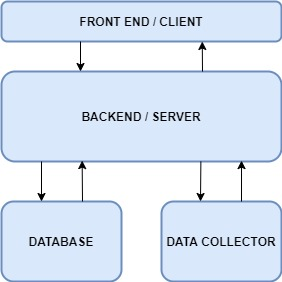
\includegraphics[width=0.4\textwidth]{images/ADS_overview.jpg}
 \caption{A simple architectural layer diagram}
\end{figure}

\subsection{Front-end Description}
%Each layer should be described separately in detail. Descriptions should include the features, functions, critical interfaces, and interactions of the layer. The description should clearly define the services that the layer provides. Also include any conventions that your team will use in describing the structure: naming conventions for layers, subsystems, modules, and data flows; interface specifications; how layers and subsystems are defined; etc. 
The front-end layer includes all software that is part of the product interface. The software is the code that is executed on the client-side (typically HTML, CSS, and JavaScript) that runs in the user's browser to create the user interface. Users interact directly with different components of the front-end, including user-entered data, buttons, links, and other features. The front-end of this application includes subsystems such as login, register, shopping list, recipes, meal planning, and shop. The front-end is designed to be accessible, pleasant, and easy to use.

\subsection{Server Description}
The back-end layer is the code that runs on the server. The back-end receives requests from the front-end (client) and contains the logic of the application to process each request and return appropriate data to the client. The back-end can directly interact with the database and data collector to retrieve the required data to fulfill each request. The back-end layer includes subsystems such as shopping manager, data parser, user management, query management, and database controller.

\subsection{Database Description}
The database layer stores and retrieves data. The database is also responsible for managing updates. The database layer includes multiple data tables that correspond with different functionalities of the product such as a table for users, meal plan, shopping list, item, item-brand, brands, recipes, and recipe ingredients.
%Having a separate database layer will allow quick and flexible access to multiple concurrent requests from the webserver. Storing the data in a database also reduces the load on the main memory of the server CPU and provides security, data backup, ensuring the integrity of data, and access to data when the server crashes.

\subsection{Data Collector Description}
The data collector layer is responsible for retrieving data from multiple sources. There is one subsystem in the data collector layer, the API Manager. The data collector retrieves data from various stores through their respective APIs and returns it to the backend layer.

